% Path diagram of the latent curve model with structured residuals (vignette lcm-sr).
\documentclass[tikz, border = 6pt]{standalone}
\usepackage{amsmath}
\usepackage{bm}
\usetikzlibrary{arrows.meta, positioning, calc}
\tikzset{
  lat/.style = {circle, draw, thick, minimum size = 12mm, inner sep = 0pt},
  obs/.style = {rectangle, draw, thick, minimum size = 10mm, inner sep = 1pt},
  noise/.style = {circle, draw, minimum size = 7mm, inner sep = 0pt},
  reg/.style = {-{Stealth[length = 2.5mm]}, thick},
  cov/.style = {{Stealth[length = 2mm]}-{Stealth[length = 2mm]}},
  lab/.style = {font = \footnotesize, fill = white, inner sep = 1pt},
  dots/.style = {font = \Large}
}
\begin{document}
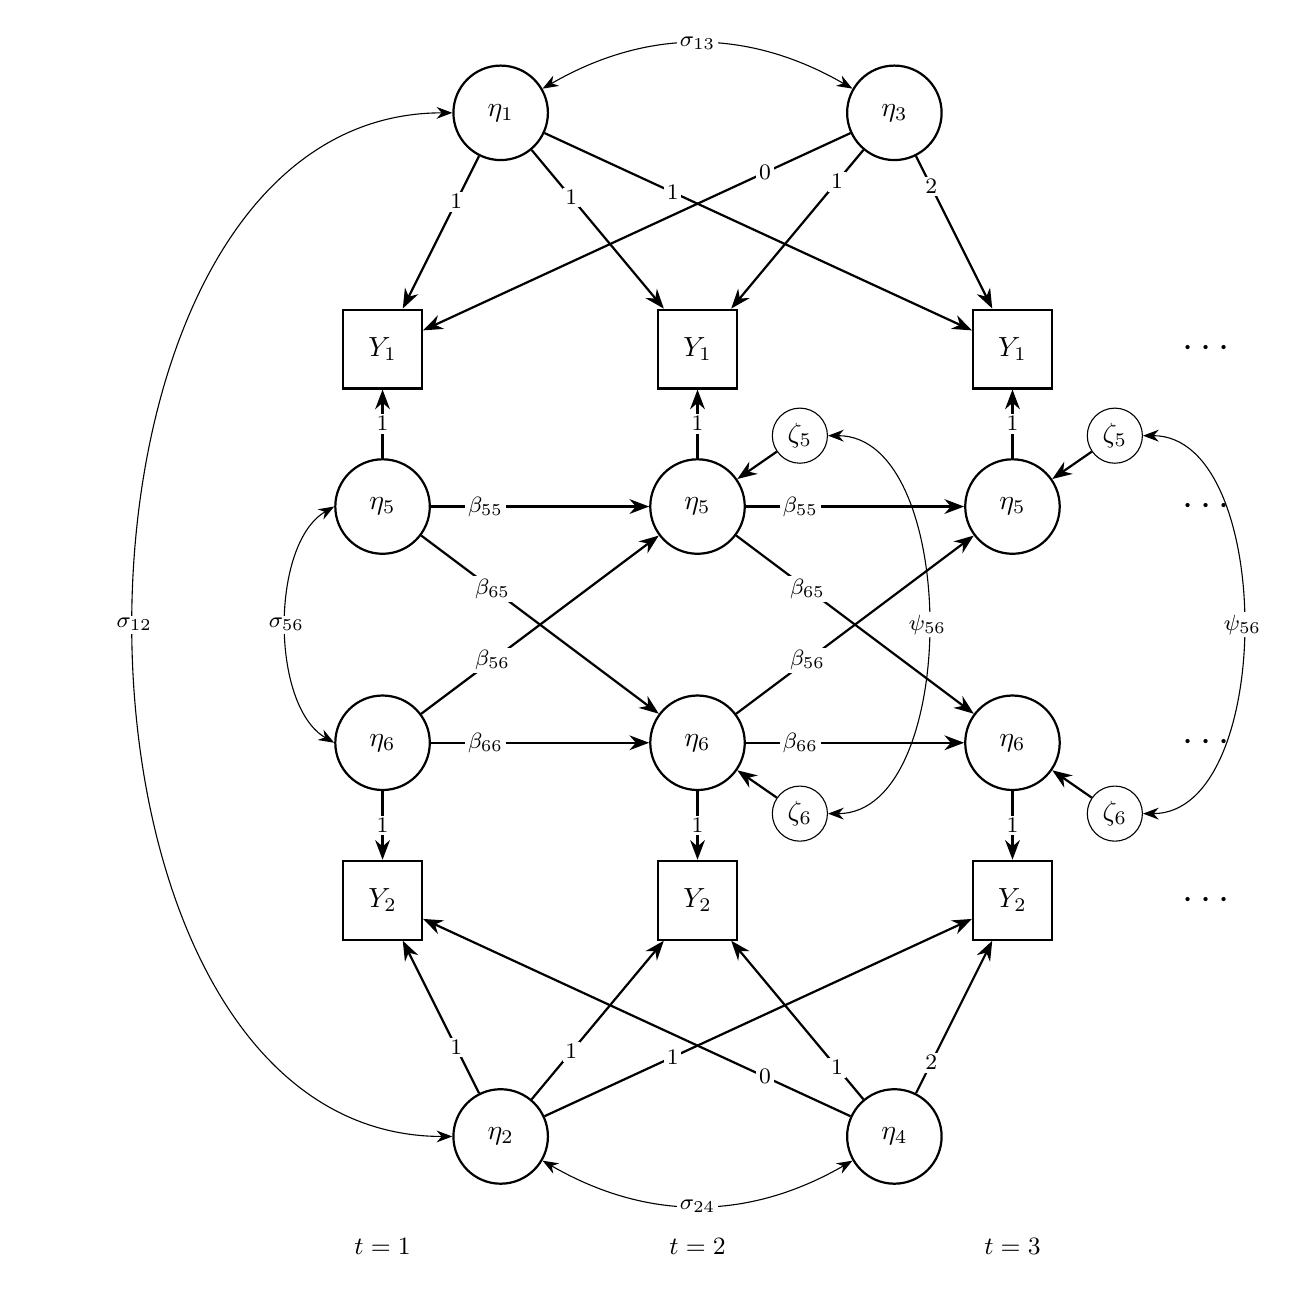
\begin{tikzpicture}
  % occasions
  \foreach \t/\x/\l in {1/0/0, 2/4/1, 3/8/2} {
    \node[obs] (y1\t) at (\x, 2) {$Y_{1}$};
    \node[lat] (w1\t) at (\x, 0) {$\eta_{5}$};
    \node[lat] (w2\t) at (\x, -3) {$\eta_{6}$};
    \node[obs] (y2\t) at (\x, -5) {$Y_{2}$};
    \draw[reg] (w1\t) -- node[lab] {1} (y1\t);
    \draw[reg] (w2\t) -- node[lab] {1} (y2\t);
    \node[font = \small] at (\x, -9.4) {$t = \t$};
  }
  % intercepts and slopes
  \node[lat] (i1) at (1.5, 5) {$\eta_{1}$};
  \node[lat] (s1) at (6.5, 5) {$\eta_{3}$};
  \node[lat] (i2) at (1.5, -8) {$\eta_{2}$};
  \node[lat] (s2) at (6.5, -8) {$\eta_{4}$};
  \foreach \t/\l in {1/0, 2/1, 3/2} {
    \draw[reg] (i1) -- node[lab, pos = 0.3] {1} (y1\t);
    \draw[reg] (i2) -- node[lab, pos = 0.3] {1} (y2\t);
    \draw[reg] (s1) -- node[lab, pos = 0.2] {$\l$} (y1\t);
    \draw[reg] (s2) -- node[lab, pos = 0.2] {$\l$} (y2\t);
  }
  \draw[cov] (i1) to[bend left = 30] node[lab] {$\sigma_{13}$} (s1);
  \draw[cov] (i2) to[bend right = 30] node[lab] {$\sigma_{24}$} (s2);
  \draw[cov] (i1.west) .. controls (-4.5, 5) and (-4.5, -8) ..
    node[lab] {$\sigma_{12}$} (i2.west);
  % structured residuals
  \foreach \s/\t in {1/2, 2/3} {
    \draw[reg] (w1\s) -- node[lab, pos = 0.25] {$\beta_{55}$} (w1\t);
    \draw[reg] (w2\s) -- node[lab, pos = 0.25] {$\beta_{66}$} (w2\t);
    \draw[reg] (w2\s) -- node[lab, pos = 0.3] {$\beta_{56}$} (w1\t);
    \draw[reg] (w1\s) -- node[lab, pos = 0.3] {$\beta_{65}$} (w2\t);
  }
  \foreach \t/\x in {2/4, 3/8} {
    \node[noise] (z1\t) at (\x + 1.3, 0.9) {$\zeta_{5}$};
    \node[noise] (z2\t) at (\x + 1.3, -3.9) {$\zeta_{6}$};
    \draw[reg] (z1\t) -- (w1\t);
    \draw[reg] (z2\t) -- (w2\t);
    \draw[cov] (z1\t.east) to[out = 0, in = 0, looseness = 0.9]
      node[lab] {$\psi_{56}$} (z2\t.east);
  }
  \draw[cov] (w11.west) to[out = 210, in = 150, looseness = 0.8]
    node[lab] {$\sigma_{56}$} (w21.west);
  \foreach \rr in {2, 0, -3, -5} {
    \node[dots] at (10.5, \rr) {$\cdots$};
  }
\end{tikzpicture}
\end{document}
